\documentclass[]{article}
\usepackage{lmodern}
\usepackage{amssymb,amsmath}
\usepackage{ifxetex,ifluatex}
\usepackage{fixltx2e} % provides \textsubscript
\ifnum 0\ifxetex 1\fi\ifluatex 1\fi=0 % if pdftex
  \usepackage[T1]{fontenc}
  \usepackage[utf8]{inputenc}
\else % if luatex or xelatex
  \ifxetex
    \usepackage{mathspec}
  \else
    \usepackage{fontspec}
  \fi
  \defaultfontfeatures{Ligatures=TeX,Scale=MatchLowercase}
\fi
% use upquote if available, for straight quotes in verbatim environments
\IfFileExists{upquote.sty}{\usepackage{upquote}}{}
% use microtype if available
\IfFileExists{microtype.sty}{%
\usepackage{microtype}
\UseMicrotypeSet[protrusion]{basicmath} % disable protrusion for tt fonts
}{}
\usepackage[margin=1in]{geometry}
\usepackage{hyperref}
\hypersetup{unicode=true,
            pdftitle={Timing of Evaluations},
            pdfauthor={Dave Bridges},
            pdfborder={0 0 0},
            breaklinks=true}
\urlstyle{same}  % don't use monospace font for urls
\usepackage{color}
\usepackage{fancyvrb}
\newcommand{\VerbBar}{|}
\newcommand{\VERB}{\Verb[commandchars=\\\{\}]}
\DefineVerbatimEnvironment{Highlighting}{Verbatim}{commandchars=\\\{\}}
% Add ',fontsize=\small' for more characters per line
\usepackage{framed}
\definecolor{shadecolor}{RGB}{248,248,248}
\newenvironment{Shaded}{\begin{snugshade}}{\end{snugshade}}
\newcommand{\KeywordTok}[1]{\textcolor[rgb]{0.13,0.29,0.53}{\textbf{#1}}}
\newcommand{\DataTypeTok}[1]{\textcolor[rgb]{0.13,0.29,0.53}{#1}}
\newcommand{\DecValTok}[1]{\textcolor[rgb]{0.00,0.00,0.81}{#1}}
\newcommand{\BaseNTok}[1]{\textcolor[rgb]{0.00,0.00,0.81}{#1}}
\newcommand{\FloatTok}[1]{\textcolor[rgb]{0.00,0.00,0.81}{#1}}
\newcommand{\ConstantTok}[1]{\textcolor[rgb]{0.00,0.00,0.00}{#1}}
\newcommand{\CharTok}[1]{\textcolor[rgb]{0.31,0.60,0.02}{#1}}
\newcommand{\SpecialCharTok}[1]{\textcolor[rgb]{0.00,0.00,0.00}{#1}}
\newcommand{\StringTok}[1]{\textcolor[rgb]{0.31,0.60,0.02}{#1}}
\newcommand{\VerbatimStringTok}[1]{\textcolor[rgb]{0.31,0.60,0.02}{#1}}
\newcommand{\SpecialStringTok}[1]{\textcolor[rgb]{0.31,0.60,0.02}{#1}}
\newcommand{\ImportTok}[1]{#1}
\newcommand{\CommentTok}[1]{\textcolor[rgb]{0.56,0.35,0.01}{\textit{#1}}}
\newcommand{\DocumentationTok}[1]{\textcolor[rgb]{0.56,0.35,0.01}{\textbf{\textit{#1}}}}
\newcommand{\AnnotationTok}[1]{\textcolor[rgb]{0.56,0.35,0.01}{\textbf{\textit{#1}}}}
\newcommand{\CommentVarTok}[1]{\textcolor[rgb]{0.56,0.35,0.01}{\textbf{\textit{#1}}}}
\newcommand{\OtherTok}[1]{\textcolor[rgb]{0.56,0.35,0.01}{#1}}
\newcommand{\FunctionTok}[1]{\textcolor[rgb]{0.00,0.00,0.00}{#1}}
\newcommand{\VariableTok}[1]{\textcolor[rgb]{0.00,0.00,0.00}{#1}}
\newcommand{\ControlFlowTok}[1]{\textcolor[rgb]{0.13,0.29,0.53}{\textbf{#1}}}
\newcommand{\OperatorTok}[1]{\textcolor[rgb]{0.81,0.36,0.00}{\textbf{#1}}}
\newcommand{\BuiltInTok}[1]{#1}
\newcommand{\ExtensionTok}[1]{#1}
\newcommand{\PreprocessorTok}[1]{\textcolor[rgb]{0.56,0.35,0.01}{\textit{#1}}}
\newcommand{\AttributeTok}[1]{\textcolor[rgb]{0.77,0.63,0.00}{#1}}
\newcommand{\RegionMarkerTok}[1]{#1}
\newcommand{\InformationTok}[1]{\textcolor[rgb]{0.56,0.35,0.01}{\textbf{\textit{#1}}}}
\newcommand{\WarningTok}[1]{\textcolor[rgb]{0.56,0.35,0.01}{\textbf{\textit{#1}}}}
\newcommand{\AlertTok}[1]{\textcolor[rgb]{0.94,0.16,0.16}{#1}}
\newcommand{\ErrorTok}[1]{\textcolor[rgb]{0.64,0.00,0.00}{\textbf{#1}}}
\newcommand{\NormalTok}[1]{#1}
\usepackage{longtable,booktabs}
\usepackage{graphicx,grffile}
\makeatletter
\def\maxwidth{\ifdim\Gin@nat@width>\linewidth\linewidth\else\Gin@nat@width\fi}
\def\maxheight{\ifdim\Gin@nat@height>\textheight\textheight\else\Gin@nat@height\fi}
\makeatother
% Scale images if necessary, so that they will not overflow the page
% margins by default, and it is still possible to overwrite the defaults
% using explicit options in \includegraphics[width, height, ...]{}
\setkeys{Gin}{width=\maxwidth,height=\maxheight,keepaspectratio}
\IfFileExists{parskip.sty}{%
\usepackage{parskip}
}{% else
\setlength{\parindent}{0pt}
\setlength{\parskip}{6pt plus 2pt minus 1pt}
}
\setlength{\emergencystretch}{3em}  % prevent overfull lines
\providecommand{\tightlist}{%
  \setlength{\itemsep}{0pt}\setlength{\parskip}{0pt}}
\setcounter{secnumdepth}{0}
% Redefines (sub)paragraphs to behave more like sections
\ifx\paragraph\undefined\else
\let\oldparagraph\paragraph
\renewcommand{\paragraph}[1]{\oldparagraph{#1}\mbox{}}
\fi
\ifx\subparagraph\undefined\else
\let\oldsubparagraph\subparagraph
\renewcommand{\subparagraph}[1]{\oldsubparagraph{#1}\mbox{}}
\fi

%%% Use protect on footnotes to avoid problems with footnotes in titles
\let\rmarkdownfootnote\footnote%
\def\footnote{\protect\rmarkdownfootnote}

%%% Change title format to be more compact
\usepackage{titling}

% Create subtitle command for use in maketitle
\newcommand{\subtitle}[1]{
  \posttitle{
    \begin{center}\large#1\end{center}
    }
}

\setlength{\droptitle}{-2em}

  \title{Timing of Evaluations}
    \pretitle{\vspace{\droptitle}\centering\huge}
  \posttitle{\par}
    \author{Dave Bridges}
    \preauthor{\centering\large\emph}
  \postauthor{\par}
      \predate{\centering\large\emph}
  \postdate{\par}
    \date{July 17, 2018}


\begin{document}
\maketitle

{
\setcounter{tocdepth}{2}
\tableofcontents
}
\subsection{Data Import}\label{data-import}

Exported \textbf{Assignment Type Summaries} from GradeCraft and
imported.

\begin{Shaded}
\begin{Highlighting}[]
\KeywordTok{library}\NormalTok{(readr)}
\KeywordTok{library}\NormalTok{(dplyr)}
\KeywordTok{library}\NormalTok{(tidyr)}
\NormalTok{datafile <-}\StringTok{ 'Principles of Nutritional Sciences Submissions - 2018-07-17.csv'}

\KeywordTok{library}\NormalTok{(readr)}
\NormalTok{dataset <-}\StringTok{ }\KeywordTok{read_csv}\NormalTok{(datafile, }\DataTypeTok{col_types=}
                      \KeywordTok{cols}\NormalTok{(}\StringTok{`}\DataTypeTok{Assignment Type}\StringTok{`}\NormalTok{ =}\StringTok{ }\KeywordTok{col_factor}\NormalTok{(}\DataTypeTok{levels=}\OtherTok{NULL}\NormalTok{)))}

\NormalTok{dropped.students <-}\StringTok{ }\KeywordTok{c}\NormalTok{(}\StringTok{'dave.bridges'}\NormalTok{,}\StringTok{'ajian'}\NormalTok{,}\StringTok{'zhongyli'}\NormalTok{)}

\NormalTok{dataset <-}\StringTok{ }\KeywordTok{separate}\NormalTok{(dataset, }\StringTok{`}\DataTypeTok{Updated At}\StringTok{`}\NormalTok{, }\DataTypeTok{sep=}\StringTok{","}\NormalTok{, }\DataTypeTok{into=}\KeywordTok{c}\NormalTok{(}\StringTok{'Day'}\NormalTok{,}\StringTok{'Date'}\NormalTok{,}\StringTok{'Time'}\NormalTok{))}

\KeywordTok{library}\NormalTok{(lubridate)}
\CommentTok{#converted dates}
\NormalTok{dataset}\OperatorTok{$}\NormalTok{Date.Year <-}\StringTok{ }\KeywordTok{paste}\NormalTok{(dataset}\OperatorTok{$}\NormalTok{Date, }\StringTok{', 2017'}\NormalTok{, }\DataTypeTok{sep=}\StringTok{""}\NormalTok{) }
\NormalTok{dataset}\OperatorTok{$}\NormalTok{Date.Year <-}\StringTok{ }\KeywordTok{mdy}\NormalTok{(dataset}\OperatorTok{$}\NormalTok{Date.Year)}

\CommentTok{#calculated cumulative sum of scores by date}
\NormalTok{sum.scores <-}
\StringTok{  }\NormalTok{dataset }\OperatorTok
\StringTok{  }\KeywordTok{group_by}\NormalTok{(Date.Year) }\OperatorTok
\StringTok{  }\KeywordTok{summarize}\NormalTok{(}\DataTypeTok{Points.Awarded =} \KeywordTok{sum}\NormalTok{(Score),}
            \DataTypeTok{Assignments.Graded =} \KeywordTok{length}\NormalTok{(Score)) }\OperatorTok
\StringTok{  }\KeywordTok{mutate}\NormalTok{(}\DataTypeTok{Total.Points =} \KeywordTok{cumsum}\NormalTok{(Points.Awarded))}
\end{Highlighting}
\end{Shaded}

\subsection{Assignments Graded Over
Time}\label{assignments-graded-over-time}

\begin{Shaded}
\begin{Highlighting}[]
\KeywordTok{library}\NormalTok{(ggplot2)}

\KeywordTok{ggplot}\NormalTok{(sum.scores, }\KeywordTok{aes}\NormalTok{(}\DataTypeTok{y=}\NormalTok{Assignments.Graded,}\DataTypeTok{x=}\NormalTok{Date.Year)) }\OperatorTok{+}
\StringTok{  }\KeywordTok{geom_point}\NormalTok{() }\OperatorTok{+}
\StringTok{  }\KeywordTok{geom_smooth}\NormalTok{() }\OperatorTok{+}
\StringTok{  }\KeywordTok{labs}\NormalTok{(}\DataTypeTok{y=}\StringTok{"Assignments per Day"}\NormalTok{,}
       \DataTypeTok{x=}\StringTok{"Date"}\NormalTok{,}
       \DataTypeTok{title=}\StringTok{"Assignments Graded Over the Semester"}\NormalTok{)}
\end{Highlighting}
\end{Shaded}

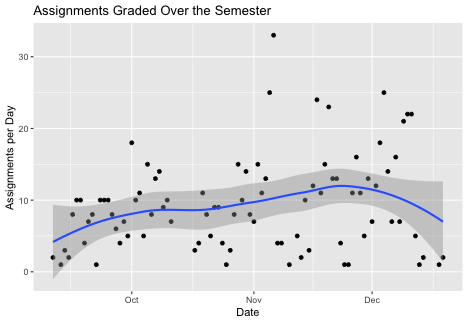
\includegraphics{figures/assignments-graded-1.png}

\begin{Shaded}
\begin{Highlighting}[]
\KeywordTok{summary}\NormalTok{(sum.scores}\OperatorTok{$}\NormalTok{Assignments.Graded) }\OperatorTok\StringTok{ }\NormalTok{broom}\OperatorTok{::}\KeywordTok{tidy}\NormalTok{() }\OperatorTok\StringTok{ }\KeywordTok{kable}\NormalTok{(}\DataTypeTok{caption=}\StringTok{"Summary Statistics for Assignments Graded Per Day"}\NormalTok{)}
\end{Highlighting}
\end{Shaded}

\begin{longtable}[]{@{}rrrrrr@{}}
\caption{Summary Statistics for Assignments Graded Per
Day}\tabularnewline
\toprule
minimum & q1 & median & mean & q3 & maximum\tabularnewline
\midrule
\endfirsthead
\toprule
minimum & q1 & median & mean & q3 & maximum\tabularnewline
\midrule
\endhead
1 & 4 & 8 & 9.39 & 13 & 33\tabularnewline
\bottomrule
\end{longtable}

\begin{Shaded}
\begin{Highlighting}[]
\KeywordTok{ggplot}\NormalTok{(sum.scores, }\KeywordTok{aes}\NormalTok{(}\DataTypeTok{x=}\NormalTok{Assignments.Graded)) }\OperatorTok{+}
\StringTok{  }\KeywordTok{geom_density}\NormalTok{(}\DataTypeTok{fill=}\StringTok{'blue'}\NormalTok{) }\OperatorTok{+}
\StringTok{  }\KeywordTok{labs}\NormalTok{(}\DataTypeTok{x=}\StringTok{"Assignments Graded Per Day"}\NormalTok{)}
\end{Highlighting}
\end{Shaded}

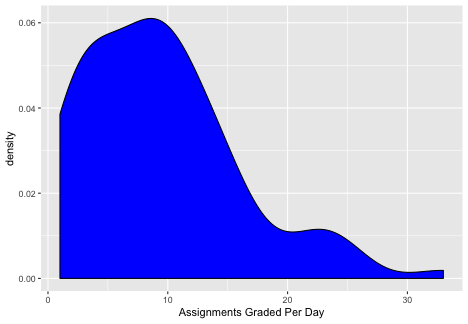
\includegraphics{figures/assignments-graded-2.png}

\subsection{Points Earned Over Time}\label{points-earned-over-time}

\begin{Shaded}
\begin{Highlighting}[]
\KeywordTok{ggplot}\NormalTok{(sum.scores, }\KeywordTok{aes}\NormalTok{(}\DataTypeTok{y=}\NormalTok{Points.Awarded,}\DataTypeTok{x=}\NormalTok{Date.Year)) }\OperatorTok{+}
\StringTok{  }\KeywordTok{geom_point}\NormalTok{() }\OperatorTok{+}
\StringTok{  }\KeywordTok{geom_smooth}\NormalTok{() }\OperatorTok{+}
\StringTok{  }\KeywordTok{labs}\NormalTok{(}\DataTypeTok{y=}\StringTok{"Cumulative Points Awarded"}\NormalTok{,}
       \DataTypeTok{x=}\StringTok{"Date"}\NormalTok{,}
       \DataTypeTok{title=}\StringTok{"Points Earned from Optional Assignments Over the Semester"}\NormalTok{)}
\end{Highlighting}
\end{Shaded}

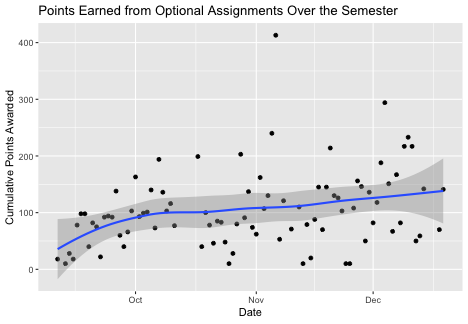
\includegraphics{figures/submitted-assignments-1.png}

\begin{Shaded}
\begin{Highlighting}[]
\KeywordTok{ggplot}\NormalTok{(sum.scores, }\KeywordTok{aes}\NormalTok{(}\DataTypeTok{y=}\NormalTok{Total.Points,}\DataTypeTok{x=}\NormalTok{Date.Year)) }\OperatorTok{+}
\StringTok{  }\KeywordTok{geom_point}\NormalTok{() }\OperatorTok{+}
\StringTok{  }\KeywordTok{geom_smooth}\NormalTok{() }\OperatorTok{+}
\StringTok{  }\KeywordTok{labs}\NormalTok{(}\DataTypeTok{y=}\StringTok{"Cumulative Points Awarded"}\NormalTok{,}
       \DataTypeTok{x=}\StringTok{"Date"}\NormalTok{,}
       \DataTypeTok{title=}\StringTok{"Cumulative Points Earned from Optional Assignments"}\NormalTok{)}
\end{Highlighting}
\end{Shaded}

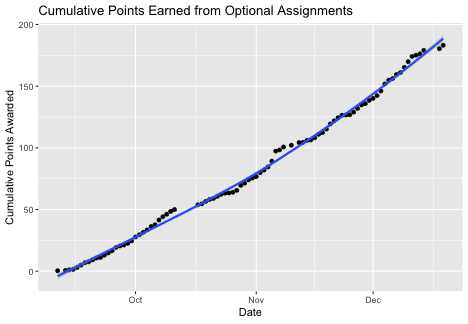
\includegraphics{figures/submitted-assignments-2.png}

\section{Session Information}\label{session-information}

\begin{Shaded}
\begin{Highlighting}[]
\KeywordTok{sessionInfo}\NormalTok{()}
\end{Highlighting}
\end{Shaded}

\begin{verbatim}
## R version 3.5.0 (2018-04-23)
## Platform: x86_64-apple-darwin15.6.0 (64-bit)
## Running under: macOS High Sierra 10.13.5
## 
## Matrix products: default
## BLAS: /Library/Frameworks/R.framework/Versions/3.5/Resources/lib/libRblas.0.dylib
## LAPACK: /Library/Frameworks/R.framework/Versions/3.5/Resources/lib/libRlapack.dylib
## 
## locale:
## [1] en_US.UTF-8/en_US.UTF-8/en_US.UTF-8/C/en_US.UTF-8/en_US.UTF-8
## 
## attached base packages:
## [1] stats     graphics  grDevices utils     datasets  methods   base     
## 
## other attached packages:
## [1] ggplot2_3.0.0   bindrcpp_0.2.2  lubridate_1.7.4 tidyr_0.8.1    
## [5] dplyr_0.7.6     readr_1.1.1     knitr_1.20     
## 
## loaded via a namespace (and not attached):
##  [1] Rcpp_0.12.17     highr_0.7        pillar_1.2.3     compiler_3.5.0  
##  [5] plyr_1.8.4       bindr_0.1.1      tools_3.5.0      digest_0.6.15   
##  [9] evaluate_0.10.1  tibble_1.4.2     gtable_0.2.0     nlme_3.1-137    
## [13] lattice_0.20-35  pkgconfig_2.0.1  rlang_0.2.1      psych_1.8.4     
## [17] parallel_3.5.0   yaml_2.1.19      withr_2.1.2      stringr_1.3.1   
## [21] hms_0.4.2        rprojroot_1.3-2  grid_3.5.0       tidyselect_0.2.4
## [25] glue_1.2.0       R6_2.2.2         foreign_0.8-70   rmarkdown_1.10  
## [29] reshape2_1.4.3   purrr_0.2.5      magrittr_1.5     backports_1.1.2 
## [33] scales_0.5.0     htmltools_0.3.6  mnormt_1.5-5     assertthat_0.2.0
## [37] colorspace_1.3-2 labeling_0.3     stringi_1.2.3    lazyeval_0.2.1  
## [41] munsell_0.5.0    broom_0.4.5
\end{verbatim}


\end{document}
